\resetdatestamp

\chapter{Introduction}

\begin{quote}
``Most principles of design should be greeted with some skepticism, for word authority can dominate our vision, and we may come to see only through the lenses of word authority rather than with our own eyes.

What is to be sought in designs for the display of information is the clear portrayal of complexity. Not the complication of the simple; rather the task of the designer is to give visual access to the subtle and the difficult - that is,

the revelation of the complex." - Edward R. Tufte, 2001 \cite{tuft2001}
\end{quote}

\section{Project Overview}

The goal of this research project is to apply a thorough understanding of a specific problem and a selection of theoretical principles in the areas of user interface design, data visualization, and human cognition to design a user interface that allows a user to solve this problem as effectively as possible. The problem addressed here is creating a mapping between a large number of signal sources and destinations distributed over many devices on a network to be used in a musical scenario. 

This research is an offshoot of a branch of research that began with the McGill Digital Orchestra Project \cite{orchestra2010}. The spirit and intent of the Digital Orchestra Project is understood as follows.

\begin{quote}
``Although designers of Digital Musical Instruments (DMI) are interested in creating useful, flexible, and creatively-inspiring interfaces and sounds, this process often depends on the vision and insight of a single individual. The McGill Digital Orchestra project instead brings together research-creators and researchers in performance, composition and music technology to work collaboratively in creating tools for live performance with digital technology." \cite{Malloch2007}
\end{quote}

The research project described in this thesis is a rethink of one particular aspect of the Digital Orchestra Project that is especially important.

\begin{quote}
``In the process of creating instruments for this project, we have found ourselves faced with the unique challenge of mapping new instruments in collaboration with experienced performers, as well as with composers tasked with writing pieces for these instruments. Because this ambitious project has taken on these three main challenges of the digital performance medium simultaneously, we have found ourselves in need of tools to help optimize the process. Specifically, mapping the various streams of controller output to the input parameters of synthesis engines has presented us with situations where both ease of use and flexibility were both [sic] of the utmost importance. We needed to be able to modify connections between data streams during precious engineer-composer-performer meeting time, while minimizing wasted minutes "reprogramming" our signal processing routines." \cite{Malloch2007}
\end{quote}

\begin{figure}[htb]
\centering
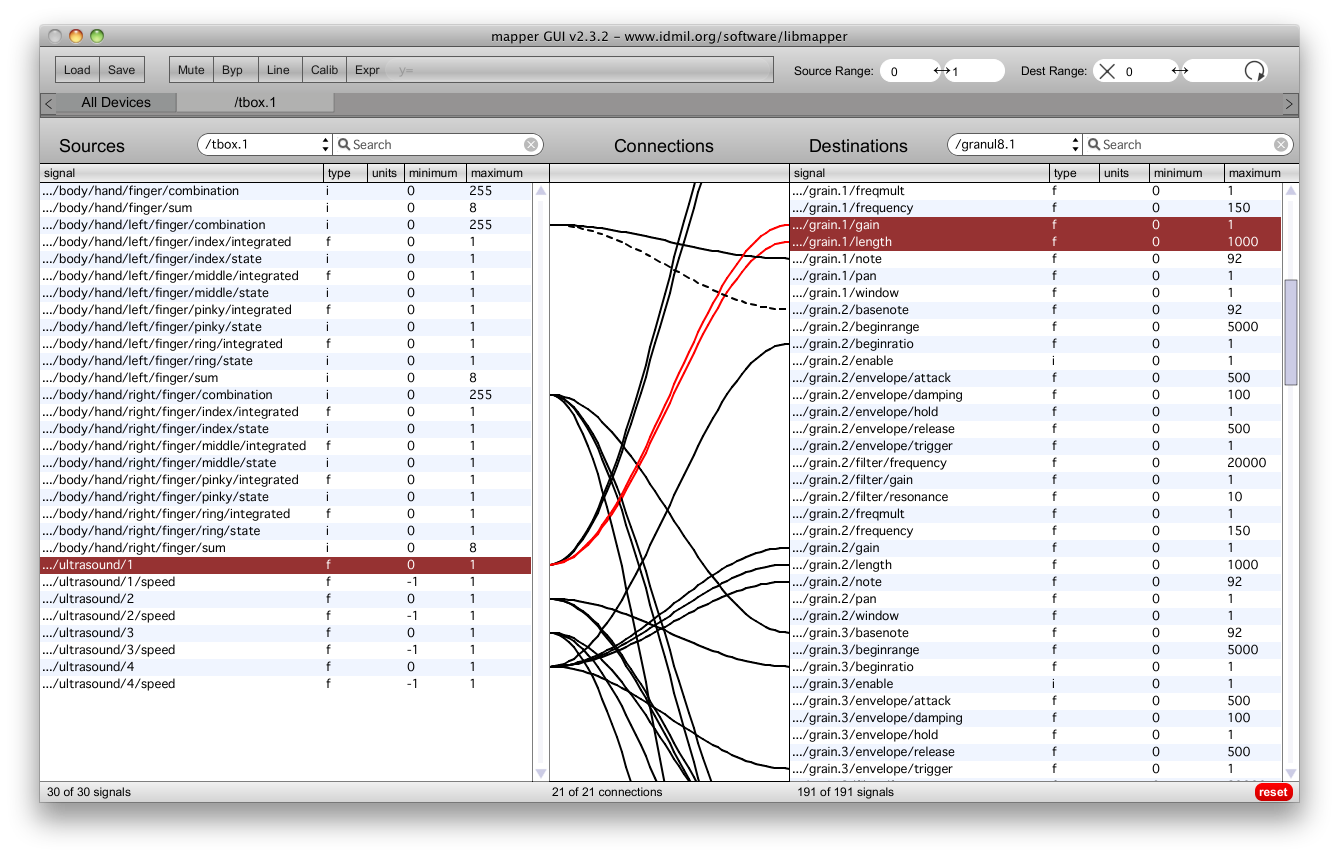
\includegraphics[width=1.0\textwidth]{maxmapper.png}
\caption{The Maxmapper GUI}
\label{fig:maxmapper}
\end{figure}

This portion of the Digital Orchestra Project is now referred to, at the Input Devices and Music Interaction Laboratory (IDMIL) at McGill University, as the \emph{Mapping Tools} project and includes the \emph{Digital Orchestra Toolbox} developed during the Digital Orchestra Project. The current manifestation of this research into simplifying DMI mapping is \emph{Libmapper}, a C library that implements the \emph{Mapper protocol} that is used to create mappings and the \emph{Maxmapper} graphical user interface (GUI) that is used to interface with the functionality that Libmapper provides. This GUI is called Maxmapper because it is implemented using the Max/MSP development environment and to differentiate it from \emph{Vizmapper}, the name of the alternative GUI developed through the research presented in this thesis.

The Maxmapper has been used by many musicians and composers and has proven its ability to simplify the DMI mapping task for non-programmers. However, the interface is typically used in situations where there are a small number of DMIs each with a small number of signals. Examining the interface in Figure \ref{fig:maxmapper}, it is clear that in a scenario with an order of magnitude more signals, the way that the data is \emph{visualized} will cease to provide the user with any understanding about the relational structure of a Mapper network or what configuration to use for a large network. Since the primary utility of a computer (in the sense of a being something that performs computations) is dealing with large bases of data and operating large numbers of things, this is a significant shortcoming of the user interface. After all, people performed computations before computers! We use computers because they can perform operations faster and in larger quantities than a human.

Computer systems engineers often talk about the ability of a system to \emph{scale}, meaning the ability of a system to gracefully handle an increasing number of users, machines, data stores, etc. without significant structural modifications or loss of utility. In some sense, what is happening is that the user interface and data visualization of Maxmapper does not \emph{scale} from DMIs to a larger sensor network.  The hope is that the research in this thesis contributes some insights into alleviating this interface problem and produces a successful alternative interface for configuring Mapper-based musical sensor networks.

\section{Thesis Structure}

This thesis is structured as follows:

Chapter 2 introduces the concept of mapping by providing a theoretical grounding of the concept as understood in mathematics and computer science and explains the more targeted concept of mappings in DMIs.

Chapter 3 examines the history of computer user interfaces as context for understanding a few principles discovered in the disciplines of user interface design, data visualization design, and cognitive science.

Chapter 4 uses these principles to design and implement a user interface for configuring mappings.

Chapter 5 concludes the thesis and presents hopes for future work on this topic.
